\documentclass[]{achemso}

\usepackage{amsmath}        % Equation editing using flags of \begin{align} and \end{align}
\usepackage{graphicx}       % Display figures using \includegraphics
\graphicspath{{figures/}}   % Location for figures relative to .tex file path
\usepackage{etoolbox}       % Make the bibliograph unjustified (to work around hbox errors)
\apptocmd{\thebibliography}{\raggedright}{}{}

%\usepackage{booktabs}       % Use table things like \toprule or \bottomrule
%\usepackage[table]{xcolor}  % Lets us use \rowcolors to make alternate table shading
%\usepackage{makecell}       % Allow the use of the \makecell command that lets linebreaks in table cells
%\usepackage{pdflscape}      % Enable the \begin{landscape} command

% chktex-file 36


%%%%%%%%%%%%%%%%%%%% Title/Abstract %%%%%%%%%%%%%%%%%%%%
\title{Uncertainty Benchmark (placeholder)}
\author{Kevin Tran}
\affiliation{Department of Chemical Engineering, Carnegie Mellon University, Pittsburgh, PA 15217}
\altaffiliation{These authors contributed equally to this work}
\author{Willie Neiswanger}
\affiliation{Department of Machine Learning, Carnegie Mellon University, Pittsburgh, PA 15217}
\altaffiliation{These authors contributed equally to this work}
\author{Junwoong Yoon}
\affiliation{Department of Chemical Engineering, Carnegie Mellon University, Pittsburgh, PA 15217}
\author{Eric Xing}
\affiliation{Department of Machine Learning, Carnegie Mellon University, Pittsburgh, PA 15217}
\author{Zachary W. Ulissi}
\affiliation{Department of Chemical Engineering, Carnegie Mellon University, Pittsburgh, PA 15217}
\email{zulissi@andrew.cmu.edu}

\begin{document}

%\setlength{\fboxrule}{0 pt}
%\begin{tocentry}
%    \includegraphics[width=\textwidth]{TOC/TOC.pdf}
%    This perspective discusses three common tools used in informatics research:
%    databases, surrogate modeling, and workflow managers. Although these tools are not
%    new, they are relatively new in the field of surface science and catalysis. We
%    discuss how these tools can augment and accelerate surface science research, and we
%    provide examples from both literature and our own work. We also provide our
%    perspective on when to use these tools and some best practices to follow when
%    creating them.
%\end{tocentry}

\begin{abstract}
    Abstract here.
\end{abstract}


%%%%%%%%%%%%%%%%%%%% Introduction %%%%%%%%%%%%%%%%%%%%

\section{Introduction}

\begin{enumerate}
    \item{ML/DS + catalysis\cite{Tran2018}}

    \item{Why uncertainty?}
        \begin{enumerate}
            \item{want confidence on DFT predictions themselves}
            \item{active routines}
        \end{enumerate}

    \item{Very quick overview of the paper (Figure~\ref{fig:overview})}
\end{enumerate}

\begin{figure}
    \centering
    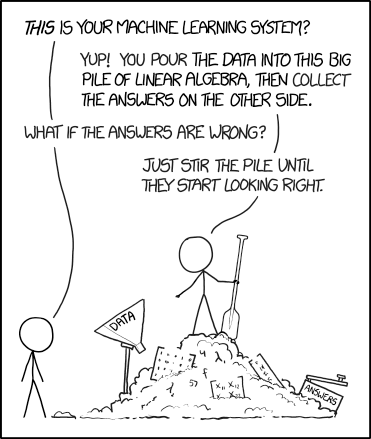
\includegraphics[width=0.5\textwidth]{placeholder.png}
    \caption{Placeholder for overview of the paper}\label{fig:overview}
\end{figure}


%%%%%%%%%%%%%%%%%%%% Methods %%%%%%%%%%%%%%%%%%%%

\section{Methods}

\begin{enumerate}
    \item{Data}
        \begin{enumerate}
            \item{GASdb}
            \item{Splits}
            \item{VASP(?)}
            \item{Blocking (on best)}
        \end{enumerate}
    \item{Modeling}
        \begin{enumerate}
            \item{CGCNN}
            \item{CGCNN Ensemble}
            \item{GP}
            \item{GP with CGCNN}
            \item{With other kernels too}
            \item{Penultimate-Fed GP}
            \item{Bayesian CGCNN with prior on weights at some layer}
            \item{Supervised error prediction (delta CGCNN)}
            \item{Dropout CGCNN}
        \end{enumerate}
    \item{Assessment}
        \begin{enumerate}
            \item{accuracy}
            \item{calibration}
            \item{sharpness}
        \end{enumerate}
\end{enumerate}

%\subsection{Assesment methods}


%%%%%%%%%%%%%%%%%%%% Results %%%%%%%%%%%%%%%%%%%%

\section{Results}

\begin{enumerate}
    \item{Table/figure of accuracies: MSE, MAE, R2, [willie get list]}
    \item{Plots:}
        \begin{enumerate}
            \item{Parity plots}
            \item{Calibration/sharpness plots}
            \item{Sharpness values per method}
        \end{enumerate}
    \item{Cost of computing each method (if it’s there)}
    \item{Human overhead and difficulty}
\end{enumerate}


%%%%%%%%%%%%%%%%%%%% Conclusions %%%%%%%%%%%%%%%%%%%%

\section{Conclusions}

Observations about relative accuracies, calibrations, sharpnesses, overhead


%%%%%%%%%%%%%%%%%%%% Misc %%%%%%%%%%%%%%%%%%%%

\section*{Code availability} Visit \texttt{https://github.com/ulissigroup/uncertainty\_benchmarking} for the code used to create the results discussed in this paper.
The code dependencies are listed inside the repository.

\section*{Author information} Corresponding author email:  zulissi@andrew.cmu.edu.
The authors declare no competing financial interest.

\section*{Acknowledgements} This research used resources of the National Energy Research Scientific Computing Center, a DOE Office of Science User Facility supported by the Office of Science of the U.S. Department of Energy under Contract No. DE-AC02-05CH11231. % chktex 8
% TODO add credit to NESAP
% TODO add credit to Willie's cluster


%%%%%%%%%%%%%%%%%%%% Bibliography %%%%%%%%%%%%%%%%%%%%

\clearpage
\bibliography{uncertainty_benchmarking}

\end{document}
